Most of the current, state-of-the-art knowledge graph completion models are based on the idea that the objects of interest can be embedded as low-dimensional, numerical vectors that can be computed effectively and efficiently by downstream models as proven in multiple other fields in the recent past, such as NLP and image processing~\cite{Wang2017KnowledgeGE}. Thereby, low-dimensional referrs to vectors limitted to a few hundred dimensions, which is low compared to comparable one-hot encodings. Equivalent to words in NLP and images in image processing, the embedded objects in KGC are a knowledge graph's entities and relations, although in practice many KGC models merely embed a graph's entities directly, while the relations' embeddings are implied, for example by the entities' relative positions to each other.

The overall process by which meaningful embeddings are created often starts with randomly initializing entity embeddings - and relation embeddings if they are represented explicitly. During training, a KGC model then repeatedly calculates the probability of facts using a scoring function that takes a fact's entity and relation embeddings as input. Thereby, the training objective is to rearrange the entity and relation embeddings so that the scoring function produces high probabilites for true facts and low probabilites for wrong facts. That rearrangement is performed by minimizing a loss function, that could be the negative of the scoring function, using backpropagation. Although most approaches see the graph under the open-world assumption, many support training by producing false facts artificially, known as \emph{negative sampling}, by corrupting true facts, i.e. replacing a true facts head or tail entity with another, random entity. Thereby, chances are high to generate a truly false fact that helps with discriminating true and false facts. At the end of training, the knowledge graph is embedded in a way that captures the structure of the original graph and can be used for further reasoning via cheap vector operations.

Various KGC models differ in their choice of a concrete embedding space, whether and how they embed relations as well as the kind of scoring function they use. As for the embedding space, many models embed the graph in a real-valued, euclidean space, whereas other models chose complex or non-euclidean spaces. Concerning relations, some models embed them implicitly as the relative position between entity embeddings, while others assign vectors, matrices or even tensors to each relation. Finally, models differ in whether they use a distance-based or a similarity-based scoring function. Overall, embedding-based KGC models can be roughly grouped into translational, tensor decomposition, neural and language models.

\begin{figure}[t]
    \centering
    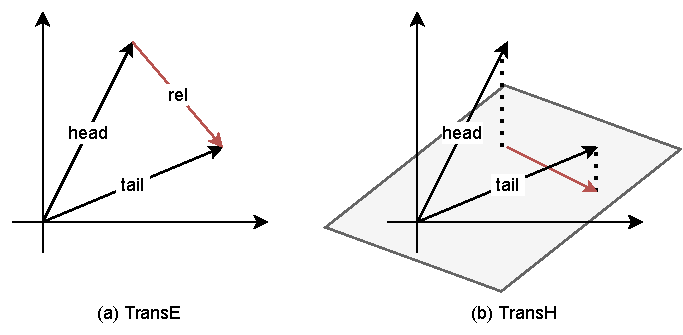
\includegraphics{3_related_work/2_embedding_based/translational}
    \caption{Concept behind translational KGC models: Relations are implicitly represented as vectors between entities - either (a) directly, as for TransE, or (b) indirectly, as for TransH, which projects entity embeddings to relation-specific hyperplanes before performing translation, which supports more complex relations.}
    \label{fig:3_related_work/2_embedding_based/translational}
\end{figure}

From the different kind of models, translational models might be the most intuitive ones. The first and simplest one is TransE~\cite{Bordes2013TranslatingEF} whose basic idea is similar to the concept behind the language model word2vec~\cite{Mikolov2013EfficientEO}: Just like the latter embeds words such that differences between word embeddings reflect semantic relations, TransE embeds entities so that differences between entity embeddings imply relations between them. For example, in word2vec the vector between the word embeddings ``king'' and ``man'' is similar to the vector between ``queen'' and ``woman''. Analogously, in the embedding space learned by TransE, one might get from the entity embedding of ``king'' to the entity embedding of ``man'' by adding the embedding of the relation ``is royal'' to the entity ``king''. \autoref{fig:3_related_work/2_embedding_based/translational} illustrates the concept. Formally, given a fact $(\textbf{head}, \textbf{rel}, \textbf{tail})$, TransE learns embeddings such that $\textbf{head} + \textbf{rel} \approx \textbf{tail}$ if the fact is true and $\textbf{head} + \textbf{rel} \neq \textbf{tail}$ if not. It thus minimizes a loss function that aims at maximizing the score function, which is the negative distance between the predicted and the actual tail embedding:

\begin{align}
    score(\textbf{head}, \textbf{rel}, \textbf{tail}) = {- || \textbf{head} + \textbf{rel} - \textbf{tail} ||}_{2}
    \label{eq:3_related_work/2_embedding_based/trans_e}
\end{align}

Problems with TransE's simple approach arise when it comes to 1-n, n-1 and n-m relations. For example, representing the facts $(Ed, speaks, Dutch)$ as well as $(John, speaks, Dutch)$ would require the entities of Ed and John to be roughly at the same spot in embedding space, but other relations between the two might require them to be apart from each other. Also problematic are cyclic relations, such as ``married to'', because TransE learns that all relations are represented by a vector of zeros. This is where other translational models step in. TransH~\cite{Wang2014KnowledgeGE}, for example, maps the entities onto relation-specific hyperplanes as illustrated in \autoref{fig:3_related_work/2_embedding_based/translationa} before performing the translation. That way multiple entities can be projected onto the same spot on the hyperplane without being at the same location in space. Similarly, TransR~\cite{Lin2015LearningEA} maps entity embeddings into separate, relation-specific embedding spaces, while other models like RotatE~\cite{Sun2019RotatEKG} and MuPR~\cite{Balazevic2019MultirelationalPG} take another approach and work in complex or hyperbolic embedding spaces, which provide ``enough room'' for the respective relations.

\begin{figure}[t]
    \centering
    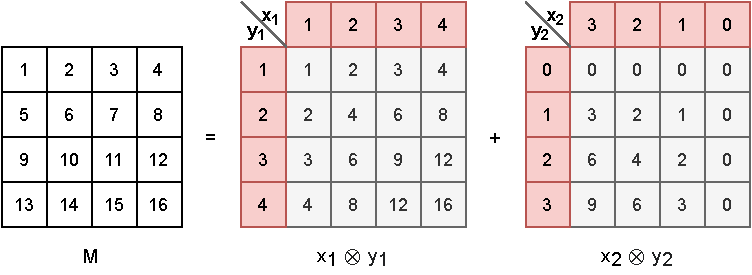
\includegraphics{3_related_work/2_embedding_based/tensor_decomposition}
    \caption{Example for tensor decomposition: A high-dimensional tensor (here, the matrix $M$) can be approximated as the sum of outer products of lower-dimensional tensors (here, the vectors $x_1$, $y_1$, $x_2$ and $y_2$).}
    \label{fig:3_related_work/2_embedding_based/tensor_decomposition}
\end{figure}

Different from translational KGC models, tensor decomposition models are based on the idea that the graph embedding space can be expressed as a composition of many smaller tensors that represent entities and relations. \autoref{fig:3_related_work/2_embedding_based/tensor_decomposition} demonstrates tensor decomposition by an example: A matrix, which is a two-dimensional tensor, can be calculated as the sum of two outer vector products between four vecctors, which are one-dimensional tensors. Likewise, a graph $G$ can be approximated by $3 \times d$ d-dimensional vectors:

\begin{align}
    G \approx \sum_{i=1}^{d} \textbf{x}_i \otimes \textbf{y}_i \otimes \textbf{z}_i
    \label{eq:3_related_work/2_embedding_based/tensor_decomposition}
\end{align}

The mathematics behind tensor decomposition can then be used to optimize the similarity-based scoring function of tensor decomposition models. For example, \autoref{eq:3_related_work/2_embedding_based/distmult} shows the score function of DistMult~\cite{Yang2015EmbeddingEA}, which corresponds to optimizing a tensor decomposition where entities and relations are represented by d-dimensional vectors.

\begin{align}
    score(\textbf{head}, \textbf{rel}, \textbf{tail}) = \sum_{i=1}^{d} \textbf{head}_i \cdot \textbf{rel}_i \cdot \textbf{tail}_i
    \label{eq:3_related_work/2_embedding_based/distmult}
\end{align}

Again, the goal of training is to find embeddings that maximize the scoring function for true facts and minimize it for false facts. Thereby, one limitation of DistMult is that its relation vectors cannot capture asymmetric relations. Other models follow different attempts to solve this problem. For example, RESCAL~\cite{Nickel2013TensorFF} represents relations using matrices instead of vectors, HolE~\cite{Nickel2016HolographicEO} leverages the non-comulativity of the correlation operators, ComplEx~\cite{Trouillon2016ComplexEF} works in complex space, and TuckER~\cite{Balazevic2019TuckERTF} employs Tucker decomposition.

\begin{figure}[t]
    \centering
    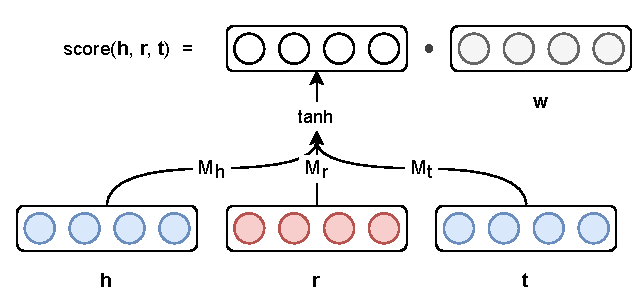
\includegraphics{3_related_work/2_embedding_based/mlp}
    \caption{Architecture of the neural MLP model~\cite{Dong2014KnowledgeVA}. In the first layer, a fact $(\textbf{h}, \textbf{r}, \textbf{t})$ is embedded using three matrices for head, relation and tail embeddings as well as the non-linear $\tanh$ function. In the second layer, the fact's score is calculated as the scalar product of the fact embedding and a weight vector $w$.}
    \label{fig:3_related_work/2_embedding_based/mlp}
\end{figure}

Yet nother approach towards KGC is followed by neural models like MLP~\cite{Dong2014KnowledgeVA} that leverage a non-linear function in a neural net to capture complex relations. \autoref{fig:3_related_work/2_embedding_based/mlp} depicts the two-layer architecture of the MLP model. At the first layer, it multiplies entity and relation vectors with three matrices it keeps for head entities, relations and tail entities before it applies the non-linear $\tanh$ activation function to the sum of resulting vectors. In the second layers follows a simple scalar multiplication with a weight vectors, yielding the final score function:

\begin{align}
    score_{MLP}(\textbf{h}, \textbf{r}, \textbf{t}) = \langle tanh(M_h \cdot \textbf{h} + M_r \cdot \textbf{r} + M_t \cdot \textbf{t}), \textbf{w} \rangle
    \label{eq:3_related_work/2_embedding_based/mlp}
\end{align}

Similar approaches include SME~\cite{Glorot2013ASM}, one of the first models to use a neural network, NTN~\cite{Socher2013ReasoningWN}, which uses relation-wise tensors before applying the non-linear function, and NAM~\cite{LIU2016ProbabilisticRV}, which employs more layers in its deep architecture.

Finally, there are KGC approaches that use the achievements of NLP models even more than tranlsational ones like TransE, in that they directly employ language models. The idea is that the variable-length sentences, consisting of words, that a language model expects as input can be replaced with variable-length paths randomly sampled from the graph, whose path segments correspond to words. Two implementations from this category include RDF2Vec~\cite{Ristoski2016RDF2VecRG}, that builds upon the word2vec~\cite{Mikolov2013EfficientEO} language model, and KGloVE~\cite{Cochez2017GlobalRV}, which is based on GloVE~\cite{Pennington2014GloveGV}.
